\section{Experiments}\label{experiment}

%Our experiments aim to answer the following three questions: (1) Can agents learn diverse behaviors with our novel neural network architecture and intrinsic reward? (2) Can our policy representation structure with the L1 regularization term balance share required by completing joint tasks? (3) Can the combination of our novelties efficiently catalyze the learning of sophisticated cooperation strategies? 

In Sec.~\ref{sec:how_work}, we use a toy game to illustrate how our approach adaptively balances experience sharing and identity-aware diversity. In this section, we use challenging tasks from GRF and SMAC benchmark to further demonstrate and illustrate the outperformance of our approach. We compare our approach against multi-agent value-based methods (QMIX~\cite{rashid2018qmix}, QPLEX~\cite{wang2020qplex}), variational exploration (MAVEN~\cite{mahajan2019maven}), and individuality emergence (EOI~\cite{jiang2020emergence}) methods. Different from baselines, we do not include agents' identification in inputs when calculating local Q-functions. We show the average and variance of the performance for our method, baselines, and ablations tested with five random seeds.
% The solid lines in all experiments are average episode returns with five random seeds for each model, and the light color areas are the error bar.
% \begin{table}[ht]
% \caption{Baseline algorithms.}
% \begin{tabular}{lll}
% \hline & Alg. & Description 
% \\ \hline & QMIX & \cite{rashid2018qmix}
% \\ Related & MAVEN & \cite{mahajan2019maven}
% \\ Works & QPLEX & \cite{wang2020qplex}
% \\ & ROMA & \cite{wang2020roma}
% \\ \hline & CDS-RAW1 & $\beta_1$ equals to zero
% \\ Abla- & CDS-RAW2& $\beta_2$ equals to zero
% \\ tions & CDS-no-$r_2^i$& $r_2^i$ equals to zero
% \\ & CDS-SA & sharing all neural networks
% \\ & &  between agents 
% \\ \hline
% \label{table1}
% \end{tabular}
% \end{table}

%\subsection{Performance on Diversity Toy Game}
%\label{sec:exp_toy}

%\begin{wrapfigure}[12]{r}{0.4\linewidth}
%	\centering
%	\vspace{-1.cm}
%	\includegraphics[width=\linewidth]{pic/pacmen_per.pdf}
%	\caption{Comparison of our approach against baseline algorithms on $\mathtt{Pacmen}$.}
%	\label{fig:pacmen_compare}
%\end{wrapfigure}

%\begin{figure}[ht]
%	\centering
%	\includegraphics[width=1.\linewidth]{pic/pacmen_per.pdf}
%	\caption{\textbf{Left:} Distributions of agents’ positions after trained by QMIX (left) and our approach (right). Parameter sharing induces similar behaviors, leading to suboptimal policies in \mathtt{Pac-Men} environment. Our approach demonstrates the potential to solve this problem with diversity. \textbf{Middle:} Comparison of our approach against baseline algorithms. \textbf{Right:} Ratios between independent and shared parts of absolute decomposed action-value functions with different $\lambda$ while learning.}
%	\label{fig:pecman}
%\end{figure}



%\includegraphics[height=0.31\linewidth]{pic/pacmen_plot}
%\includegraphics[height=0.31\linewidth]{pic/pacmen-large}

%We compare our approach with baselines in the environment introduced in Sec.~\ref{sec:how_work}. As shown in Fig.~\ref{fig:pacmen_compare}, our approach outperforms all the baselines by a wide margin. When baselines mislead agents to cluster for completing resources, our approach encourages agents to scatter in different rooms to eat dots for continuously obtaining rewards. MAVEN shows diversity for eating two rounds of dots (get 20 episode return by 5M). But the comparison demonstrates that our approach with identity-aware exploration outperforms joint trajectories aware exploration, which is more tricky to optimize. The comparison between ROMA maintains our analysis in Sec.~\ref{relate}. Because all agents are all initialized at the maze center with similar observation, it is difficult for ROMA to emerge agents with different roles to explore the environment.

%Comparing the performance of three different $\lambda$, which controls the weight of the L1 regularization term, we notice lower L1 regularization weight leads to better performance, because this environment urgently needs diversity among agents. With the best $\lambda$, our approach outperforms all the baselines by a wide margin. The final policy is visualized on the left side of Fig.~\ref{fig:pecman}. When baselines such as QMIX mislead agents to cluster for completing resources, our approach encourages agents to scatter in different rooms to eat dots for continuously obtaining rewards. MAVEN shows diversity for eating two rounds of dots (get 20 episode return by 5M). But the comparison demonstrates that our approach with identity-aware exploration outperforms joint trajectories aware exploration, which is more tricky to optimize. The comparison between ROMA maintains our analysis in Sec.~\ref{relate}. Because all agents are all initialized at the maze center with similar observation, it is difficult for ROMA to emerge agents with different roles to explore the environment.

%By scattered in different rooms to eat dots, agents can continuously get rewards, which demonstrates our approach has a reliable ability to encourage agents to behave differently to find more opportunities. 

%Meanwhile, as shown in the right side of Fig.~\ref{fig:pecman}, we demonstrate ratios between the absolute value of independent action-value functions and shared action-value functions with different $\lambda$ while learning. We notice higher L1 regularization weight leads to a lower ratio.

\subsection{Performance on Google Research Football (GRF)}\label{sec:exp_grf}



\begin{figure*}[ht]
\centering
\includegraphics[width=1.\linewidth]{pic/GRF.pdf}
\caption{Comparison of our approach against baseline algorithms on Google Research Football.}
\label{fig:grf_result}
\end{figure*}


We first benchmark our approach on three challenging Google Research Football (GRF) offensive scenarios $\mathtt{academy\_3\_vs\_1\_with\_keeper}$, $\mathtt{academy\_counterattack\_hard}$, and our own designed full-field scenario $\mathtt{3\_vs\_1\_with\_keeper\ (full\ field)}$. Agents' initial locations for each scenario are shown in Appendix~\ref{sec:grf_scen}. In GRF tasks, agents need to coordinate timing and positions for organizing offense to seize fleeting opportunities, and only scoring leads to rewards. In our experiments, we control left-side players (in yellow) except the goalkeeper. The right-side players are rule-based bots controlled by the game engine. Agents have a discrete action space of 19, including moving in eight directions, sliding, shooting, and passing. The observation contains the positions and moving directions of the ego-agent, other agents, and the ball. The $z$-coordinate of the ball is also included. We make a small and reasonable change to the half-court offensive scenarios: our players will lose if they or the ball returns to our half-court. All baselines and ablations are tested with this modification. Environmental reward only occurs at the end of the game. They will get +100 if they win, else get -1.



We show the performance comparison against baselines in Fig.~\ref{fig:grf_result}. Our approach outperforms all the scenarios. MAVEN needs more time to explore sophisticated strategies, demonstrating that \name~incentives more efficient exploration. EOI lets each agent consider individuality and cooperation simultaneously by setting local learning objectives but without exclusive Q networks, making cooperation and individuality hard to be persistently coordinated. In comparison, taking advantage of the partially shared network structure, \name~agents learn diverse but coordinated strategies. For example, as shown in Fig.~\ref{fig:teaser}, three agents have different behaviors, with the first agent passing the ball, the second scoring, while the third running to threaten. These diverse behaviors closely coordinate, forming a perfect scoring strategy and leading to significant outperformance against EOI. 

%Influence-based approaches EITI and EDTI can learn effective strategies. However, these two methods use the sum of all pairwise interaction values between agents, which brings more computational complexity, causing less efficient learning than our approach.

%Role-based learning method ROMA attempts to learn diverse roles, which shares similarity in spirit with our method. However, since the role encoder of ROMA is shared among agents and is conditioned on local observations, ROMA struggles in complex Google Research Football tasks. 

%Comparing our approach's performances between three scenarios indicates that our approach needs more training to balance individuality and group tasks when the problem space increases. We plan to explore how to improve the scalability of our approach in future works for more complex scenarios with more agents.



%It is the fastest method to explore practical strategies and continuously improve the winning rate throughout training. 

%\begin{figure*}[ht]
%\centering
%\includegraphics[width=1.\linewidth]{pic/grf_long.pdf}
%\caption{Why does our approach work? The balance between identity-aware diversity and homogeneity encourages sophisticated strategies.}
%\label{fig:process}
%\end{figure*}
%Correspondence between the learning performance and diversity/cooperation balance achieved by our method during the training process.

% diverse distributed exploration /  / diverse & cooperative teams
%\textbf{How does \name~work?} We further visualize the development of team performance, accompanied by the balancing process between identity-aware diversity and homogeneity, to show why our method works (Fig.~\ref{fig:process}). We pinpoint three critical points during the training process. In the first training stage ($0\sim 1.2$M), \name~players attempt to be as diverse as possible due to the sparsity of environmental rewards. Agents behave differently, such as sliding randomly (Fig.~\ref{fig:process}a) or running aimlessly (Fig.~\ref{fig:process}b). These behaviors essentially promote distributed exploration. After $T = 1.2$M, agents realize they need to organize an offense to score a goal. They aggregate near the goal and prepare to attack while dribbling. However, in this second training phase, agents focus on the ball rather than cooperation, leading to unnecessary competition. For example, as highlighted by the circle in Fig.~\ref{fig:process}c and Fig.~\ref{fig:process}d, our players try to compete for the ball. They lose their individuality after obtaining huge benefits brought by scoring. We believe this is also why some baseline algorithms, such QMIX and QPLEX, encounter a performance bottleneck in GRF scenarios. After $T = 3$M, our approach gradually achieves the balance of diversity and cooperation and again enables players to make diverse decisions when handling the ball for better collaboration. The whole training process shows our approach can coordinate the relationship between agents while keeping a good balance between individuality and group tasks.
% In \mathtt{3vs2} scenario, we also visualize our approach's training process in detail, as shown in Fig.~\ref{grf result}. 

\subsection{Performance on StarCraft II}\label{sec:exp_sc2}
% Our approach performs well in the diversity test. And we hope diversity can be a catalyst for more efficient cooperation. In Section~\ref{sec:exp_sc2} and ~\ref{sec:exp_grf}, we will demonstrate how our approach pushes the forward state of the art on the StarCraft II micromanagement benchmarks and Google Research Football scenarios.

\begin{figure*}[ht]
\centering
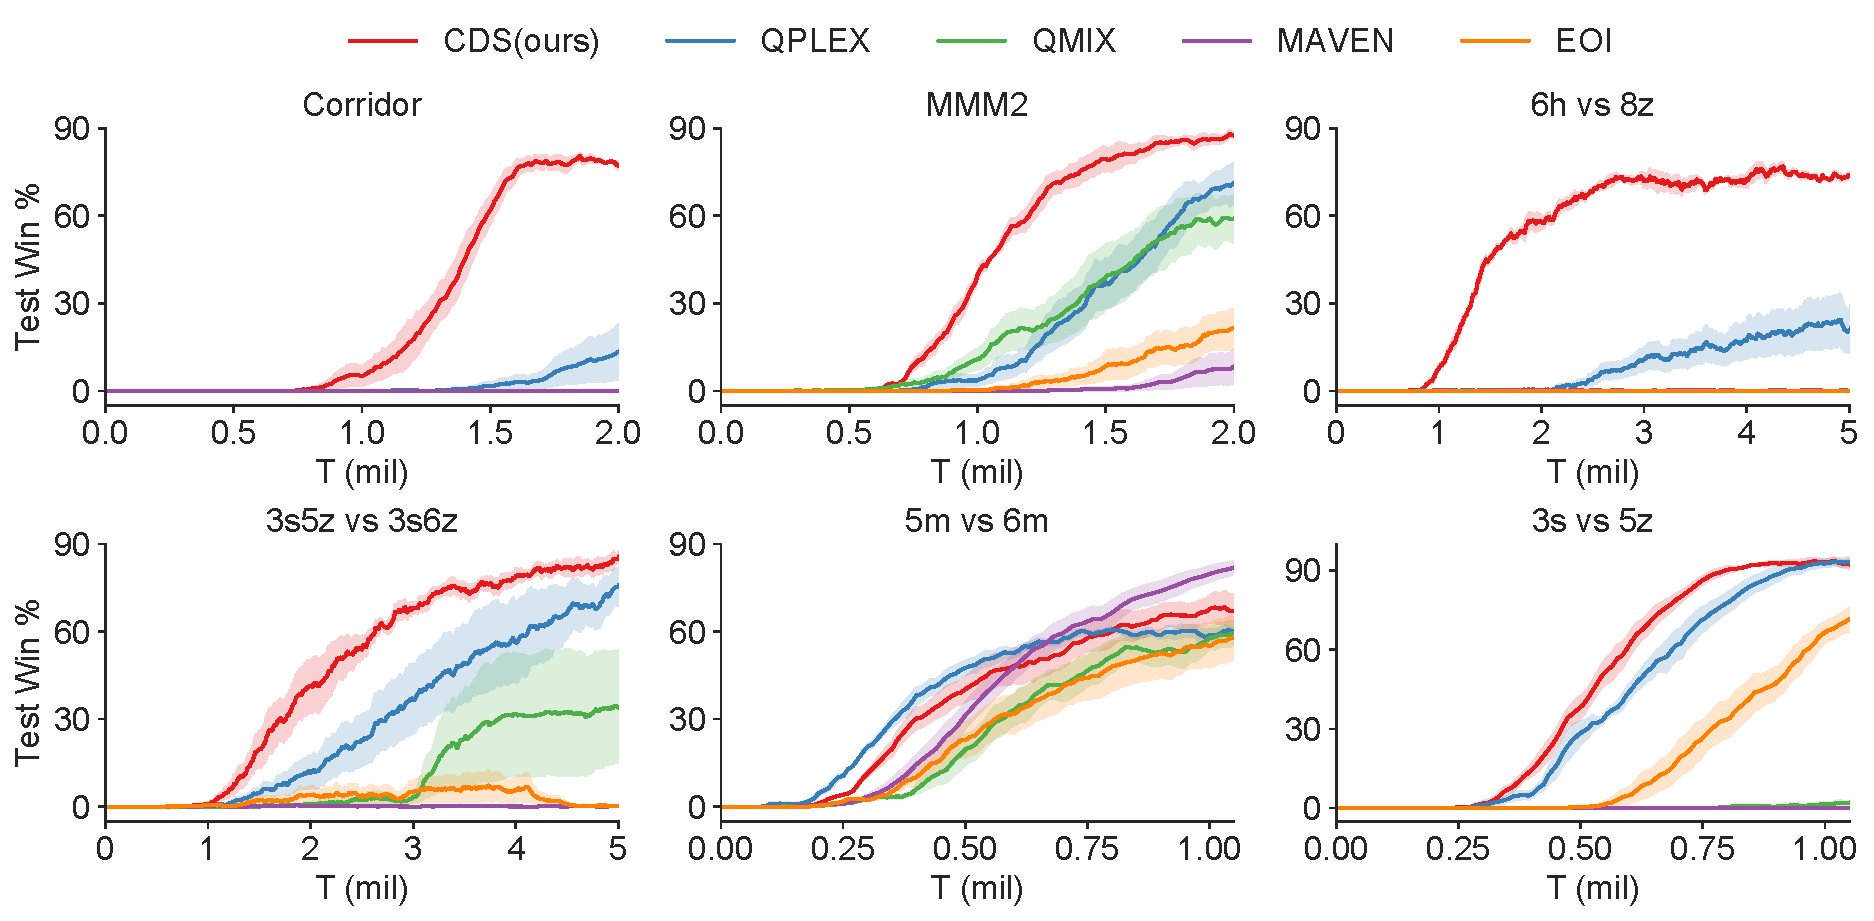
\includegraphics[width=1.\linewidth]{pic/SC2.pdf}
\caption{Comparison of our approach against baseline algorithms on four \textbf{super hard} SMAC maps: $\mathtt{corridor}$, $\mathtt{MMM2}$, $\mathtt{6h\_vs\_8z}$, and $\mathtt{3s5z\_vs\_3s6z}$ and two \textbf{hard} SMAC maps: $\mathtt{5m\_vs\_6m}$ and $\mathtt{3s\_vs\_5z}$.}
\label{fig:sc2_result}
\end{figure*}

In this section, we test our approach on the StarCraft II micromanagement (SMAC) benchmarks~\cite{samvelyan2019starcraft}. This benchmark consists of various maps classified as easy, hard, and super hard. Here we test our method on four super hard maps: $\mathtt{corridor}$, $\mathtt{MMM2}$, $\mathtt{6h\_vs\_8z}$, and $\mathtt{3s5z\_vs\_3s6z}$, and two hard SMAC maps: $\mathtt{5m\_vs\_6m}$ and $\mathtt{3s\_vs\_5z}$. For the four super hard maps, our approach outperforms all baselines with acceptable variance across random seeds, as shown in Fig.~\ref{fig:sc2_result}. The baselines QPLEX and QMIX can achieve satisfactory performance on some challenging benchmarks, such as $\mathtt{3s5z\_vs\_3s6z}$ and $\mathtt{MMM2}$. But on other maps, they need the proposed diversity-celebrating method to get better performance. Compared with MAVEN and EOI, our approach maintains its out-performance with the balance between diversity and homogeneity for learning sophisticated cooperation. Our approach performs similarly with baselines for the two hard maps, indicating our balancing process may not improve the learning efficiency in environments that require pure homogeneity. But for challenging environments, where sophisticated strategies are laborious to explore, our approach can efficiently search for valuable strategies with stable updates.


%Comparing our approach with MAVEN shows that our approach is much more efficient in completing complex tasks. 

%EOI behaves worse than QPLEX, and the cooperation even collapses on $\mathtt{3s5z\_vs\_3s6z}$. This observation shows that, compared to EOI, CDS incentivizes diverse behaviors which are more cooperative in terms of task solving. 

%EITI behaves worse than QPLEX, while EDTI achieves outstanding performance on $\mathtt{3s5z\_vs\_3s6z}$, where our approach achieves similar performance at the end of training. Taking the value of interaction into consideration lets EDTI better facilitate exploration. But the same as EITI, EDTI needs to sum up all the pairwise influence between agents, which is complex to calculate. Our approach simplifies the computational complexity by encouraging agents to highlight themselves from other agents, bypassing calculating pairwise influence. In this way, our approach can be adapted to multi-agent problems of larger scales.



\subsection{Ablations and Visualization}
\label{exp:ab}


To understand the contribution of each component in the proposed \name~framework, we carry out ablation studies to test the contribution of its three main components: Identity-aware \emph{diversity} (A) encouragement and \emph{partially shared} (B) neural network structure with \emph{L1 regularization} (C) on non-shared Q-functions. To test component A, we ablate our intrinsic rewards to four different levels. (1) CDS-Raw ablates all intrinsic rewards by setting $\beta$ in Eq.~\ref{Eq:TD} to zero. (2) CDS-No-Identity ablates $H\left(\tau_{T} | i d\right)$ and only optimize $H\left(\tau_{T} \right)$ in Eq.~\ref{equ:mutual_information} by setting $\beta_1$ in Eq.~\ref{final reward} to zero. (3) CDS-No-Action ablates item \raisebox{.5pt}{\textcircled{\raisebox{-.9pt}{2}}} in Eq.~\ref{equ:per_timestep} by setting $\beta_2$ in Eq.~\ref{final reward} to zero. (4) CDS-No-Obs ablates item \raisebox{.5pt}{\textcircled{\raisebox{-.9pt}{3}}} in Eq.~\ref{equ:per_timestep} by ablating $\beta_{1} \log q_{\phi}\left(o_{t+1} | \tau_{t}, a_{t}, i d\right)-\log p\left(o_{t+1} | \tau_{t}, a_{t}\right)$ in Eq.~\ref{final reward}. To test component B, we design CDS-All-Shared, which ablates independent action-value functions together with the L1 loss and, like baselines, adds agents' identification to the input. To test component C, we design CDS-No-L1, which ablates L1 regularization terms by setting $\lambda$ in Eq.~\ref{eq:final_optimize} to zero.
%the following ablation studies: (1) CDS-RAW ablates the diversity-encouraging intrinsic rewards. (2) CDS-RAW1 simplifies intrinsic reward by setting $\beta_1$ to zero. (3) CDS-RAW2 simplifies intrinsic reward by setting $\beta_2$ to zero. (4) CDS-no-TranDiverse simplifies intrinsic reward by setting term \textcircled{3} in Eq.~\ref{equ:per_timestep} to zero, which indicates transition diversity. (5) CDS-All-Shared ablates $\mathcal{L}_{L_{1}}\left(Q^{I}(\theta_a^I)\right)$ together with the independent action-value functions and add agents' id to the input. (6) CDS-no-L1 only ablates $\mathcal{L}_{L_{1}}\left(Q^{I}(\theta_a^I)\right)$.

\begin{figure*}[ht]
\centering
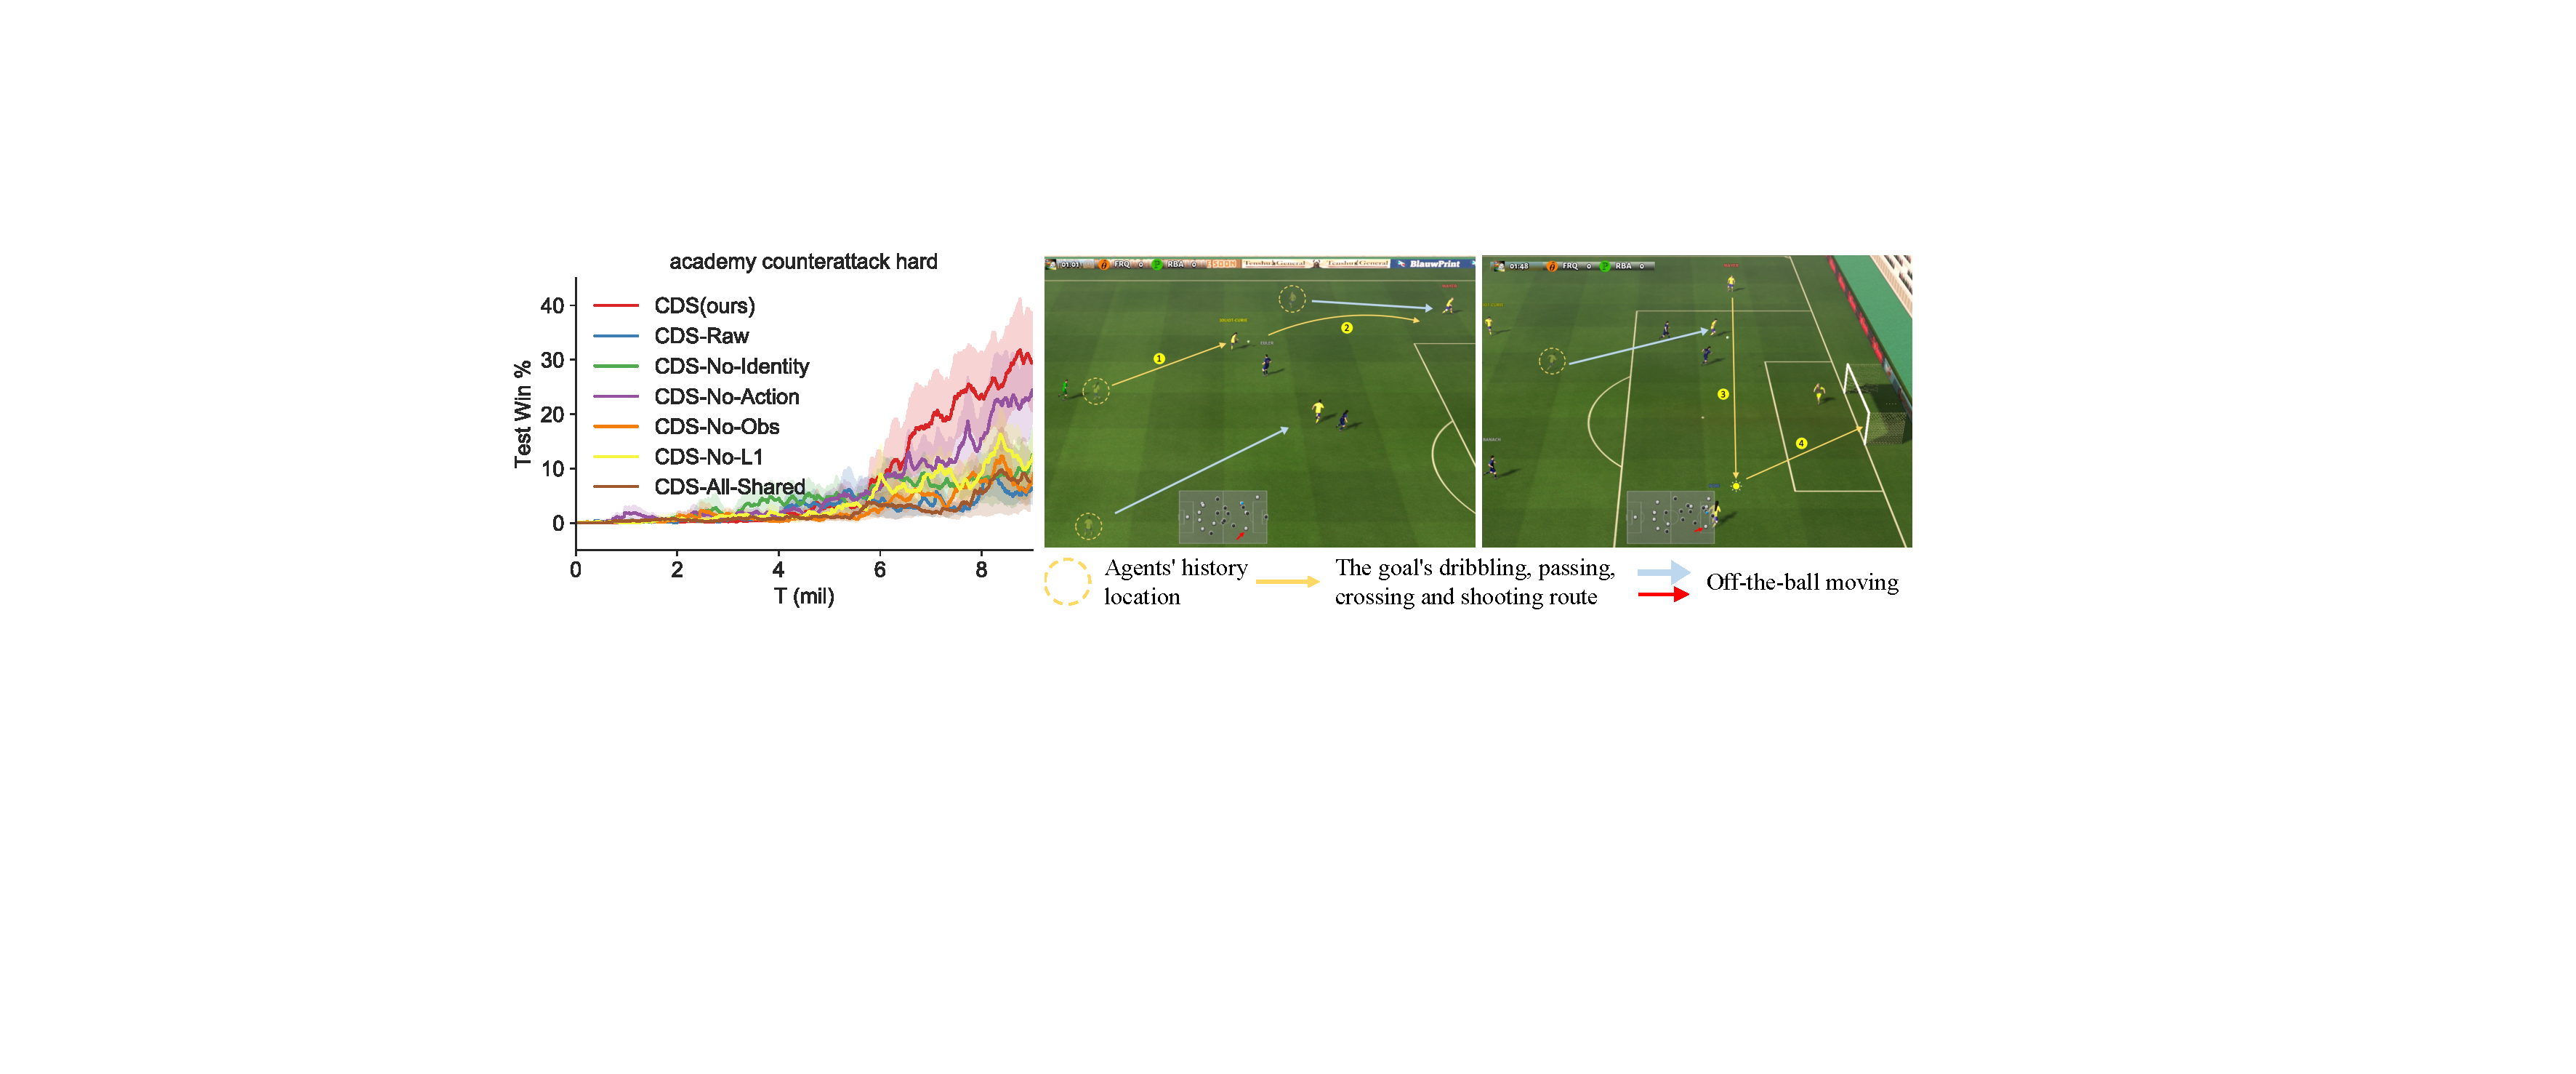
\includegraphics[width=1.\linewidth]{pic/grf_ab.pdf}
\caption{\textbf{Left.} Ablation studies on $\mathtt{academy\_counterattack\_hard}$. \textbf{Right.} Visualization of trained policies, which achieve complex cooperation with impressive off-the-ball moving strategies.}
\label{Ablation_GRF}
\end{figure*}

We first carry out ablation studies on $\mathtt{academy\_counterattack\_hard}$ to analyze which part of our novelties lead to the outstanding performance as shown on the left side of Fig.~\ref{Ablation_GRF}. The ablation of each part of our intrinsic reward will bring a noticeable decrease in performance. Among them, the least impact on performance is the ablation of action-aware diversity. CDS-No-L1 performs similarly to MAVEN, which indicates that unlimited diversity is harmful to cooperation. CDS-All-Shared performs even worse than QPLEX, demonstrating that identity-aware diversity is difficult to emerge without our specially designed network structure.

%. As , CDS-No-Identity performs the best among all ablations. However, compared with CDS, CDS-No-Identity is slower to explore winning strategy and performs noticeably worse at the end of training. Thus for the intrinsic reward component in this environment, the superior performance of CDS is primarily due to optimizing group diversity. Still, the specialization of agents' behavior given identification noticeably improves learning. Moreover, the performance of  CDS-No-Obs and CDS-Raw perform poorly. CDS-No-Action performs a little better but is similar to QPLEX. Therefore, action- and observation-aware diversity are both crucial. 

% including CDS-no-BehaviorDiverse and CDS-no-TranDiverse
%Therefore each agent can help improve learning in GRF scenarios.


%although group diversity is more critical in GRF than single agent's identity, encouraging agents to find their special responsibility can achieve more stable and efficient learning. The poor performance of CDS-RAW implies that only maintaining policy representation diversity is not enough. Specific catalysts are needed to guide the diversity of agents for novel ideas to share. Meanwhile, the comparison between CDS and CDS-no-L1 demonstrates the L1 regularization term's significant role in encouraging agents to share their knowledge actively and be diverse only when necessary.

We further visualize the final trained strategies on the right side of Fig.~\ref{Ablation_GRF}, which shows complex cooperation between agents. Our players first attack down the wing by dribbling and passing the ball. Then one of them draws the attention of the enemy defenders and the goalkeeper, while the ball being passed across the penalty area. Another player catches the ball and completes the shot. The most impressive part of our sophisticated strategies is off-the-ball moving strategies. All agents without the ball try to use their unique and valuable moves to create more scoring opportunities, which shows behavior and position diversity for finishing the goal.


%a remarkable balance between diversity and homogeneity, leading to advanced coordination between agents.

\begin{figure*}[ht]
\centering
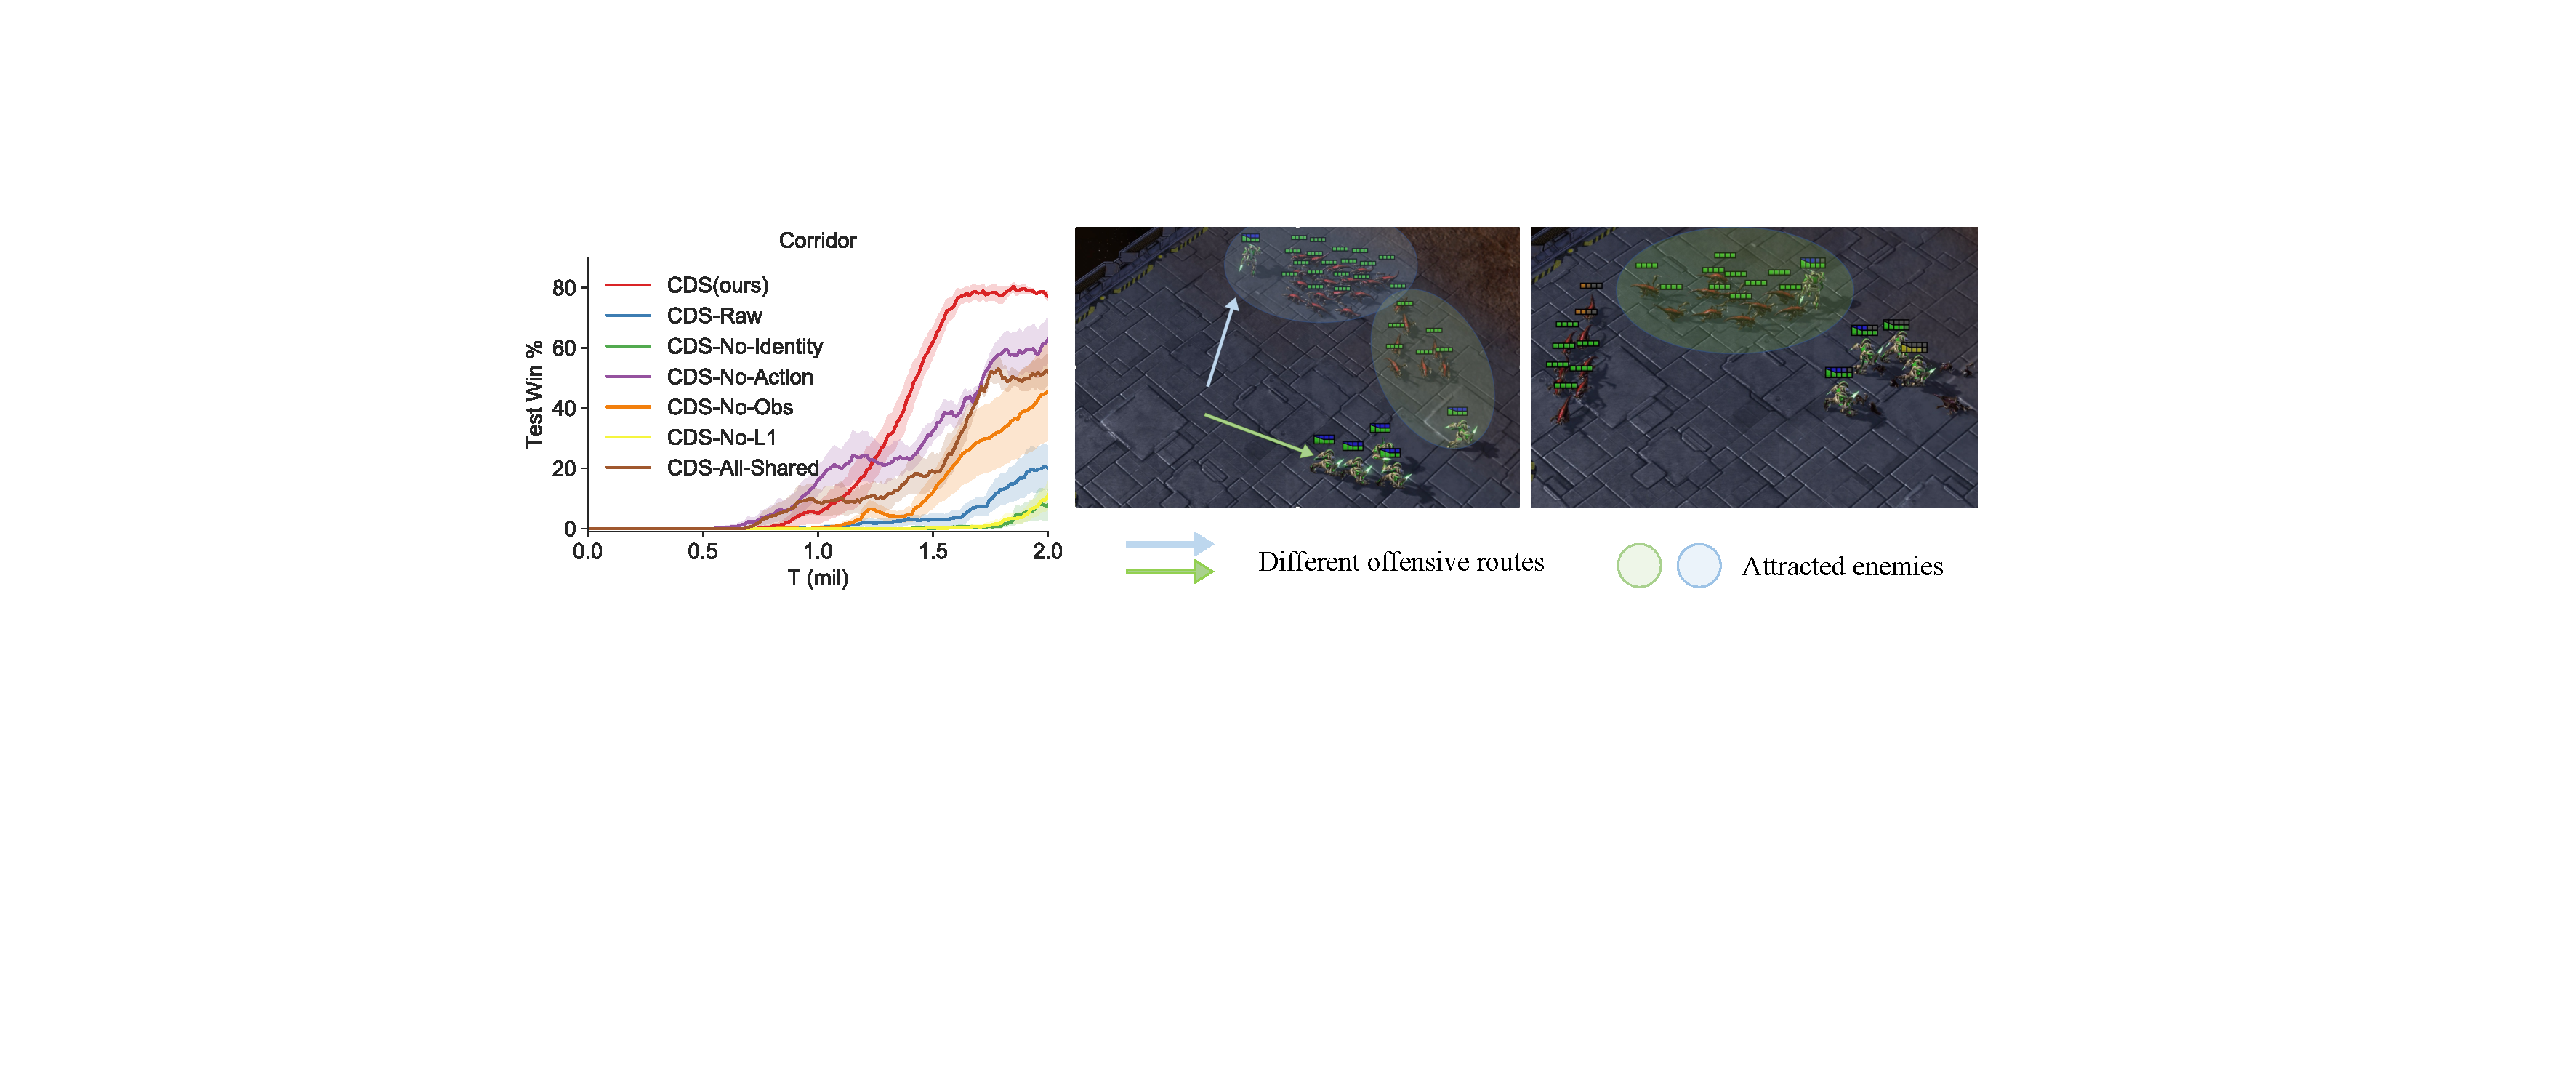
\includegraphics[width=1.\linewidth]{pic/corridor_ab.pdf}
\caption{\textbf{Left.} Ablation studies in super hard map $\mathtt{corridor}$. \textbf{Right.} Visualization of the final trained strategies, which achieves a hard-earned victory brought by the sacrifice of a warrior.}
\label{Ablation_SC}
\end{figure*}

We also carry out ablation studies on the super hard map $\mathtt{corridor}$ as shown in Fig.~\ref{Ablation_SC} left. Same as results on $\mathtt{academy\_counterattack\_hard}$, the ablation of action-aware diversity causes the least performance gap. Among all the ablations, CDS-No-L1 and CDS-No-Identity perform worst, whose performance is similar to QPLEX. This phenomenon indicates excessive diversity is harmful to the emerge of complex cooperation. CDS-All-Shared achieves acceptable performance, different from the GRF scenario, reflecting the different demand levels for the representation diversity of these two kinds of benchmarks.


%We notice considerable differences against the GRF scenario. For instance, CDS-No-Identity performs the worst on $\mathtt{corridor}$ but the best on $\mathtt{academy\_counterattack\_hard}$ among all ablations. This phenomenon indicates the different importance of group diversity and specialization of agents' behavior given identification between GRF and SMAC. For SMAC, the most important intrinsic reward component is optimizing the conditional entropy. Unlimited identity-aware diversity without L1 regularization, CDS-No-L1, has worse performances than QPLEX. Therefore, excessive diversity is harmful to the emerge of complex cooperation, which is the same in both GRF and SMAC. 

%It is because group operations is necessary in SMAC, but there must be few agents behave 




%$H(\tau)$ and $H(\tau|id)$ between GRF and SMAC: GRF needs more diversity in general trajectories, while SMAC needs more identity for each agent. It also shows the extensive adaptability of CDS. Moreover, the terrible behavior of CDS-no-L1 reiterates the significance of being diverse only when necessary. Other ablations will cause performance degradation more or less. The comparison between CDS-no-BehaviorDiverse and CDS-no-TranDiverse demonstrates that transition diversity, reflecting the consequence of behaviors, is slightly more critical than behavior diversity, which remains the same in both GRF and SMAC.

%, to demonstrate the functionality of our approach's each part. Experiment results of ablation studies are shown on the left side of Fig.~\ref{Ablation_SC}, and ablations are shown in Table~\ref{table1}. If we set $\beta_1$ to 0 in CDS-RAW1, we will only maximize $H(\tau)$ for trajectory coverage. The superiority of our approach against CDS-RAW1 highlights the importance of minimizing $H(\tau \mid id)$, which is related to agents' individuality. Setting $beta_2$ to zero in CDS-RAW2 equals to setting $r_1^i$ to zero. Comparing our approach against CDS-RAW2 demonstrates the significance of diversity in action, which will not dominate performance changes but will affect training stability. The comparison between CDS-RAW2 and CDS-no-$r_2^i$ demonstrates that $r_2^i$ has more influence on the final performance than $r_1^i$. Sharing all neural networks between agents without independent action-value function and L1 regularization will lead to noticeable performance degradation, demonstrating the significance of diversity in policy representation.

To better explain why our approach performs well. On $\mathtt{corridor}$, we also visualize the final strategies in Fig.~\ref{Ablation_SC} right. In this super hard map, six friendly Zealots are facing 24 enemy Zerglings. The disparity in quantity means our agents are doomed to lose if they attack together. One Zealot, whose route is highlighted blue, becomes a warrior leaving the team to attract the attention of most enemies in the blue oval. Although doomed to sacrifice, he brings enough time for the team to eliminate a small part of the enemies in the green oval. After that, another Zealot stands out to attract some enemies and enables teammates to eradicate them. These sophisticated strategies reflect the leverage between diversity and homogeneity by encouraging agents to be diverse only when necessary.

%In summary, combining identity-aware diversity and our structural novelties, CDS achieves new state-of-the-art on GRF scenarios and significantly outperforms baselines on the SMAC benchmark.

%\textbf{Our approach can balance diversity and homogeneity for sophisticated strategies, but needs more training for leading diversity to solve tasks when the problem space increases. We plan to explore how to improve the scalability of our approach in future works for more complex GRF scenarios.}

%Comparing our approach's performances between three scenarios indicates that our approach needs more training to balance individuality and group tasks when the problem space increases. We plan to explore how to improve the scalability of our approach in future works for more complex scenarios with more agents.
%If Zealots involve in the battle directly after spawning, they will be defeated because of the disadvantage in number. The middle picture demonstrates that one Zealot becomes a warrior leaving the team to attract most enemies' attention. His route and the enemies he draws are painted blue. Although destined to sacrifice, he brings enough time for the team to eliminate a small part of enemies highlighted by green. After that, another Zealot stands out to attract some enemies and enables other teammates to eradicate the others. Diversity is the key to let agents find this joint policy -- all agents need to adopt different trajectories. Meanwhile, our approach can balance diversity with a cooperative learning target so that agents are coordinated to be diverse only when necessary.
% And due to the guidance of the first warrior Zealot, the remaining enemies are out of the attack range of Zealots and enter the next area. 
%We also do experiments in the \mathtt{4vs3} scenario and show results in Fig.~\ref{grf result 2}. \mathtt{4vs3} scenario is more challenging then \mathtt{3vs2}. In \mathtt{4vs3}, all our controlled agents start from midfield instead of the penalty area and face more opponents. We notice that, in this scenario, we still outperform baselines in training stability and efficiency. MAVEN achieves performance close to our approach at 5M. But due to the unstable selection of joint policy latent variable, while chasing diversity, the performance of MAVEN declines afterward. We visualize our learned best policies in Fig.~\ref{grf result 2}, which indicates that our approach can precisely coordinate agents in time and space. In general, our approach pushes forward state of the art on two basic scenarios \mathtt{3vs2} and \mathtt{4vs3} and shows the potential to win in more complex scenarios.